% vim:spell spelllang=sk
\section{Decimácia vo frekvencii radix2}
Toto je druhý bežne používaný algoritmus pre mocniny dvojky. Je veľmi
podobný decimácii v čase, ako si ukážeme. Avšak využíva iný rozklad
transformácie. Zamerajme sa tentoraz  špeciálne na výpočet párnych a
nepárnych indexov:
\begin{equation}
    \begin{split}
    X_{2k} &= \sum_{l=0}^{n-1} x_l \omega_{n,2kl} \\
            &= \sum_{l=0}^{n/2-1} x_l \omega_{n,2kl} +
              \sum_{l=0}^{n/2-1} x_{n/2+l} \omega_{n, 2k(n/2 + l)} \\
            &= \sum_{l=0}^{n/2-1} (x_l + x_{n/2+l}) \omega_{n, 2kl} \\
            &= \sum_{l=0}^{n/2-1} (x_l + x_{n/2+l}) \omega_{n/2, kl} 
    \end{split}
\end{equation}
Podobne, pre nepárne indexy platí
\begin{equation}
    \begin{split}
    X_{2k+1} &= \sum_{l=0}^{n-1} x_l \omega_{n,(2k+1)l} \\
            &= \sum_{l=0}^{n/2-1} x_l \omega_{n,(2k+1)l} +
              \sum_{l=0}^{n/2-1} x_{n/2+l} \omega_{n, (2k+1)(n/2 + l)} \\
            &= \sum_{l=0}^{n/2-1} (x_l - x_{n/2+l}) \omega_{n, (2k+1)l} \\
            &= \sum_{l=0}^{n/2-1} ((x_l - x_{n/2+l})
              \omega_{n,l} )
            \omega_{n/2, kl}
    \end{split}
\end{equation}
Posledné riadky predchádzajúcich rovníc sa podobajú na Fourierovu
transformáciu a môžeme ich na ňu prepísať:
\begin{align}
    X_{2k} &= DFT_{n/2}[x_l + x_{n/2+l}] \\
    X_{2k+1} &= DFT_{n/2}[(x_l - x_{n/2+l}) \omega_{n,l}]
\end{align}
Butterfly diagmam pre decimáciu vo frekvencii 
znázorňujúci práve vypočítaný fakt
vidíme na obrázku \ref{fig:butterfly_dif}

\begin{figure}[htp]
    \centering
        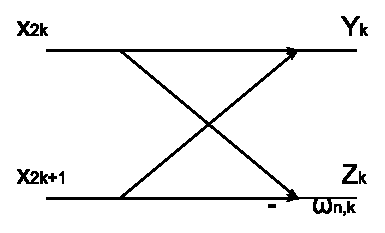
\includegraphics{obrazky/algoritmy/butterfly_dif}
        \caption{Butterfly diagram pre decimáciu vo frekvencii}
    \label{fig:butterfly_dif}
\end{figure}

Porovnaním s diagramom pre decimáciu v čase na obrázku
\ref{fig:butterfly_dit} môžeme
vidieť náramnú podobnosť. Vyzerá to tak, že butterfly pre decimáciu vo
frekvencii
je presne reverzným výpočtom butterfly pre decimáciu v čase. Toto
pozorovanie nie je náhodné, ako sa čitaťeľ môže presvedčiť. Dôsledok
je pozoruhodný - výpočet decimácie vo frekvencii 
prebieha presne v opačnom poradí
ako u decimácie v čase. Ilustrácia výpočtu pre $n=8$ sa dá nájsť na
ilustrácii \ref{fig:dif}

\begin{figure}[htp]
    \centering
        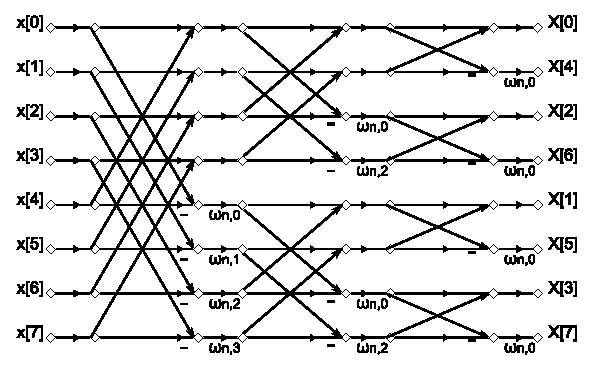
\includegraphics{obrazky/algoritmy/dif}
        \caption{Výpočet decimácie vo frekvencii pre $n=8$}
    \label{fig:dif}
\end{figure}
To, že výsledok je "bit reversed" nás neprekvapí a dôkaz je podobný
dôkazu u decimácie v čase.

\begin{python}
import cmath
import math
from bitutils import BitUtils

class DIF:
    def transformInPlace(data):
        n = len(data)
        assert(BitUtils.isPowerOf2(n))


        skip = n

        while skip >= 2:
            for block in range(n/skip):
                for i in range(skip/2):
                    # do butterfly
                    y = data[block * skip + i]
                    z = data[block * skip + skip/2 + i]
                    k = i * (n/skip)
                    twiddle = cmath.exp( -2 * 1j * math.pi / n * k)
                    data[block * skip + i] = y + z
                    data[block * skip + skip/2 +i] = (y - z) * twiddle
            skip /= 2
        BitUtils.bitReverseInPlace(data)


    transformInPlace = staticmethod(transformInPlace)
\end{python}

\todo{cite:dif}
